%%%%%%%%%%%%%%%%%%%%%%%%%%%%%%%%%%%%%%%%%%%%%%%%%%%%%%%%%%%%%%%%%%%%%%%%%%%%

\documentclass[draft]{agujournal2019}
\usepackage{url} %this package should fix any errors with URLs in refs.
% \usepackage{lineno}
\usepackage[inline]{trackchanges} %for better track changes. finalnew option will compile document with changes incorporated.
\usepackage{soul}
\usepackage{hyperref}
\usepackage{graphicx}
\usepackage{cancel}
\linenumbers
\usepackage{verbatim}
%%%%%%%
\newcommand{\detailtexcount}[1]{%
  \immediate\write18{texcount -merge -sum -q #1.tex > #1.wcdetail }%
  \verbatiminput{#1.wcdetail}%
}

\draftfalse

%% Enter journal name below.
%% Choose from this list of Journals:
%
% JGR: Atmospheres
% JGR: Biogeosciences
% JGR: Earth Surface
% JGR: Oceans
% JGR: Planets
% JGR: Solid Earth
% JGR: Space Physics
% Global Biogeochemical Cycles
% Geophysical Research Letters
% Paleoceanography and Paleoclimatology
% Radio Science
% Reviews of Geophysics
% Tectonics
% Space Weather
% Water Resources Research
% Geochemistry, Geophysics, Geosystems
% Journal of Advances in Modeling Earth Systems (JAMES)
% Earth's Future
% Earth and Space Science
% Geohealth
%
% ie, \journalname{Water Resources Research}

\journalname{A Scientific Journal}

\usepackage[utf8]{inputenc}
 
\begin{document}


\title{Overleaf Tutorial}


\authors{Manish Devana}


\correspondingauthor{=name=}{=email address=}

\begin{keypoints}
\item Easy and fully loaded latex editor (Great way to learn latex if you've been thinking about trying it out)
\item Student Pricing for Premium version 
\item Contains templates for lots of major journals
\item Mendeley integration 
\item Google Drive-like live collaboration and commenting 

\end{keypoints}


\clearpage

\section*{Contents}
\begin{enumerate}
  \item Getting Started in Overleaf
  \item Mendeley, Zotero, Github.
  \item Collaboration tools
  \item Things that don't always work that well
\end{enumerate}

\clearpage
\section{Getting Started}



Why bother with latex?

Latex for equations and math heavy writing:
\begin{eqnarray*}
        \frac{1}{n}\sin x & = & \mathrm{?} \\
        \frac{1}{\cancel{n}} \mathrm{si}\cancel{\mathrm{n}} ~x & = & \mathrm{?} \\
        \mathrm{six} & = & 6
\end{eqnarray*}

Latex separates CONTENT from STYLE/FORMATTING. i.e. You deal with the content of your work without worrying about accidentally messing with the formatting of the document. That is adjusted when you convert the latex document into a pdf (Which overleaf does for you!).

Its also faster than word... no buggy scrolling through long documents with lots of figures!


If you are not familiar with Latex, this is a good place to start: \url{https://www.overleaf.com/learn/latex/Learn_LaTeX_in_30_minutes}
\begin{enumerate}
  \item Make Account
  \item Find a template or start with a blank project.
  \item customize the editor
  \item upload figures and files to project to keep it all organized
  \item write about your amazing science
  \item Convert to pdf OR publish directly to a journal (I haven't tried this yet...)
\end{enumerate}
% \begin{figure}
% \noindent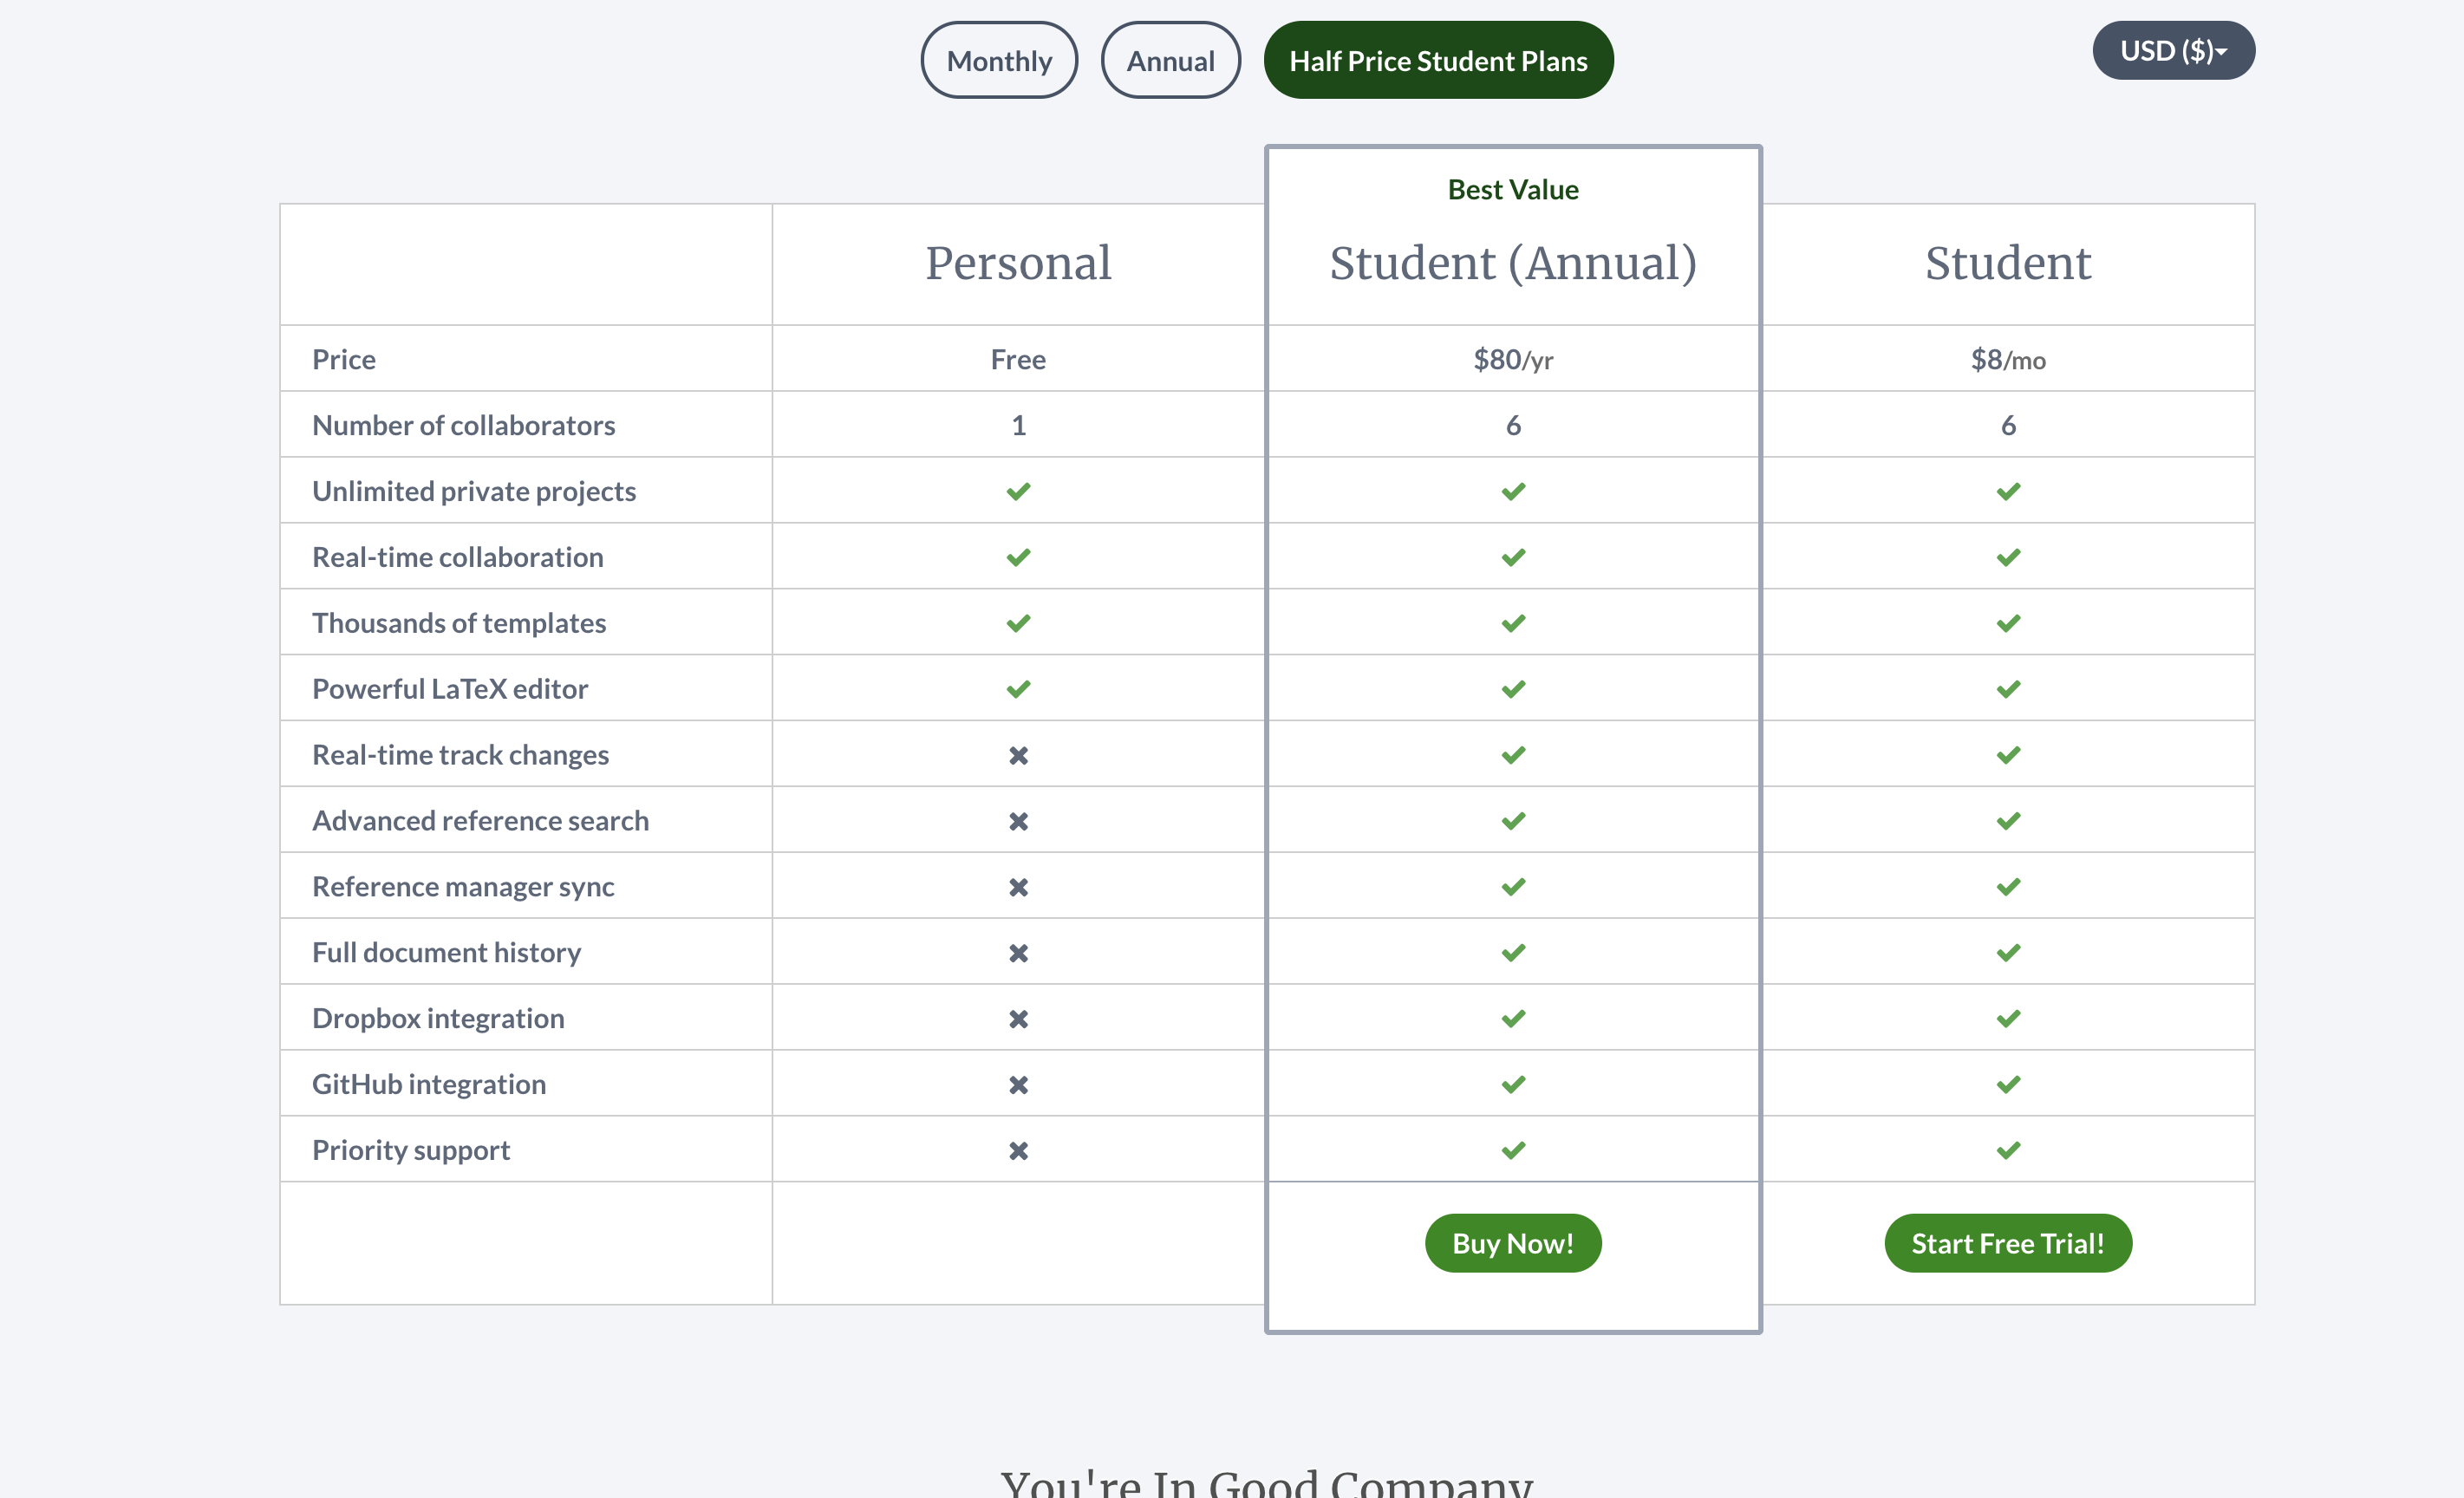
\includegraphics[width=\textwidth]{pic.png}
% \caption{ }
% \label{flame}
% \end{figure}
\clearpage


\section{Mendeley/Zotero and Github}

Sync Mendeley or Zotero Library from the "UPLOAD" screen.


Syncing your mendeley or zotero libraries is a quick and easy way to manage citations in projects. If you add new references to your library, simply click on your .bib file and resync it to update the references.  


How to use the citation: \cite{Zou2017ObservedAtlanticc} insert Citation here (search function doesnt work that well)

reference a thing \cite{Johns2019Registration:,}

There is also an option to sync the project of github and dropbox. You link your accounts in the menu bar in the top left corner of the editor.
%
\clearpage


\clearpage

\section{Collaboration Tools}
Add collaborators with the "share" button. It works similarly to google docs. 


Once you add people to work with you can see their comments and live chat with them. If you activate track changes (paid feature) then you can track , comment, and accept/reject changes by other authors.
\clearpage
\section{Things that don't always work that well}
\begin{enumerate}
  \item word count (but theres a work around)
  %%TC:ignore
\subsection*{Word Count}

% \quickwordcount{main}
% \quickcharcount{main}
\detailtexcount{main}
%%TC:endignore
  \item Reference Searching
  \item spell check is awful (I use grammarly by copying and pasting sections into grammarly)
  \item not built for working offline (can work around if you have an offline Tex editor and sync up the changes but its a pain)








  
 \end{enumerate}
\clearpage


\bibliography{references.bib}


\end{document}



